% !TEX TS-program = pdflatex
% !TEX encoding = UTF-8 Unicode

\documentclass[a4paper, titlepage=false, parskip=full-, 10pt]{scrartcl}

\usepackage[utf8]{inputenc}
\usepackage[T1]{fontenc}
\usepackage[english, ngerman]{babel}
\usepackage{babelbib}
\usepackage{hyperref}
\usepackage{listings}
\usepackage{framed}
\usepackage{color}
\usepackage{graphicx}
\usepackage[normalem]{ulem}
\usepackage{cancel}
\usepackage{amsmath}
\usepackage{amssymb}
\usepackage{amsthm}
\usepackage{algorithm}
\usepackage{algorithmic}
\usepackage{geometry}
\usepackage{subfigure}
\geometry{a4paper, top=20mm, left=35mm, right=25mm, bottom=40mm}

\newcounter{tasknbr}
\setcounter{tasknbr}{1}
\newenvironment{task}[1]{{\bf Aufgabe \arabic {tasknbr}\stepcounter{tasknbr}} (#1):\begin{enumerate}}{\end{enumerate}}
\newcommand{\subtask}[1]{\item[#1)]}

% Listings -----------------------------------------------------------------------------
\definecolor{red}{rgb}{.8,.1,.2}
\definecolor{blue}{rgb}{.2,.3,.7}
\definecolor{lightyellow}{rgb}{1.,1.,.97}
\definecolor{gray}{rgb}{.7,.7,.7}
\definecolor{darkgreen}{rgb}{0,.5,.1}
\definecolor{darkyellow}{rgb}{1.,.7,.3}
\lstloadlanguages{C++,[Objective]C,Java}
\lstset{
escapeinside={§§}{§§},
basicstyle=\ttfamily\footnotesize\mdseries,
columns=fullflexible, % typewriter font look better with fullflex
keywordstyle=\bfseries\color{blue},
% identifierstyle=\bfseries,
commentstyle=\color{darkgreen},      
stringstyle=\color{red},
numbers=left,
numberstyle=\ttfamily\scriptsize\color{gray},
% stepnumber=5,
% numberfirstline=true,
breaklines=true,
% prebreak=\\,
showstringspaces=false,
tabsize=4,
captionpos=b,
% framexrightmargin=-.2\textwidth,
float=htb,
frame=tb,
frameshape={RYR}{y}{y}{RYR},
rulecolor=\color{black},
xleftmargin=15pt,
xrightmargin=4pt,
aboveskip=\bigskipamount,
belowskip=\bigskipamount,
backgroundcolor=\color{lightyellow},
extendedchars=true,
belowcaptionskip=15pt}

%% Enter current values here: %%
\newcommand{\lecture}{Algorithmische Geometrie SS15}
\newcommand{\tutor}{}
\newcommand{\assignmentnbr}{5}
\newcommand{\students}{Julius Auer, Alexa Schlegel}
%%-------------------------------------%%

\begin{document}  
{\small \textsl{\lecture \hfill \tutor}}
\hrule
\begin{center}
\textbf{Übungsblatt \assignmentnbr}\\
[\bigskipamount]
{\small \students}
\end{center}
\hrule

\begin{task}{Suchen in ebenen Unterteilungen}
\item[]

Eine ebene Unterteilung ist eine Partition von $\mathbb{R}^2$ in durch Strecken und Strahlen begrenzte Gebiete (Einbettung eines planaren Graphen $G$)\\

Wenn man durch jeden Knoten der ebenen Unterteilung eine vertikale Linie zieht und sich dann den Schnittpunkt nach oben und unten merkt, dann entstehen ganz viele Trapze, die man dann wieder in zwei Dreiecke unterteilen kann. Was man dann davon hat keine Ahnung. Und welche Datenstruktur hier Sinn macht mit ($O(log(n))$ weiß ich auch nicht. Vielleicht ein Baum? So eine ebene Unterteilung wenns dumm läuft kann doch dann ganz ganz viele Trapeze haben oder?

Ich verstehe die Aufgabe nicht so richtig. Wir hatten in der VL auch das Thema Suche in Ebenen Unterteilungen, da haben wir aber triangulierte Unterteilungen betrachtet, wo die Außenfacette ein Dreieck ist, das Suchproblem dafür gelöst und dann einfach um es Allgmeiner zu machen, um ebene Unterteilungen die nicht so sind, ein ganz ganz großes Dreieck rundrum konstruiert und dann den Rest trianguliert.

* einfache Datenstruktur beschreiben zum Suchen mit Anfragezeit $O(\log n)$\\
* Vorverarbeitungszeit\\
* Speicherplatz für Datensturktur
\end{task}

\begin{task}{$L_1$-Voronoi-Diagramme}
\item[]
In $L_1$-Metrik beschreiben die Punkte mit Abstand $d$ von einem Punkt ein Quadrat mit Seitenlänge $2\cdot d$ (Abb. \ref{fig:l1_1}).
\begin{figure}[h]
\begin{center}
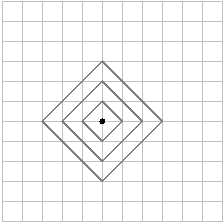
\includegraphics[width=3cm]{capture0}
\end{center}
\caption{Punkte mit Abständen 1,2,3 von einem Punkt liegen auf den Ränder dieser Quadrate}
\label{fig:l1_1}
\end{figure}

Eine zwei Voronoi-Regionen trennende Kante hat nun stets eine von drei möglichen Formen, welche vom Verhältnis zwischen der X-Differenz und der Y-Differenz der Punkte bestimmt wird. Dominiert die X-Differenz, wird die Kante senkrecht ''aussehen''. Dominiert die Y-Differenz, wird die Kante waagerecht ''aussehen''.

Es sind im Folgenden die drei Fälle abgebildet, dass bei zwei Punkten die Y-Differenz (Abb. \ref{fig:l1_2}), die X-Differenz (Abb. \ref{fig:l1_3}) oder keine der beiden (Abb. \ref{fig:l1_4}) dominiert.

Jede Abbildung zeigt die drei untergeordneten Fälle, bei denen der in der dominanten Dimension größere Punkt in der rezesiven Dimension kleiner/gleich/größer dem anderen Punkt ist. Andere Fälle als die gezeigten sieben kann es nicht geben.

\begin{figure}[h]
\begin{center}
\subfigure{
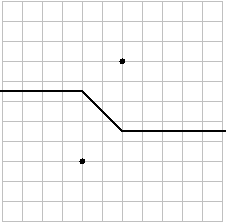
\includegraphics[width=3cm]{capture1}
}
\subfigure{
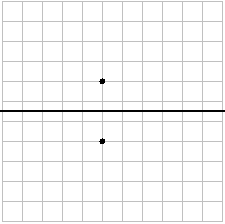
\includegraphics[width=3cm]{capture2}
}
\subfigure{
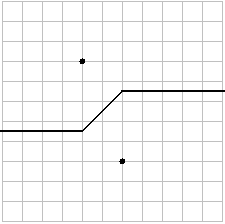
\includegraphics[width=3cm]{capture3}
}
\end{center}
\caption{Fall 1: $\left|\frac{x_1-x_2}{y_1-y_2}\right| <1$}
\label{fig:l1_2}
\end{figure}

\begin{figure}[h]
\begin{center}
\subfigure{
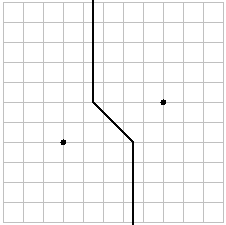
\includegraphics[width=3cm]{capture4}
}
\subfigure{
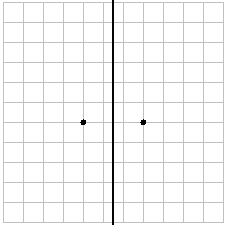
\includegraphics[width=3cm]{capture5}
}
\subfigure{
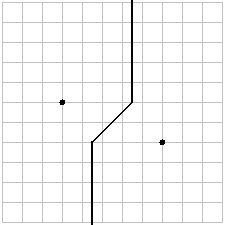
\includegraphics[width=3cm]{capture6}
}
\end{center}
\caption{Fall 2: $\left|\frac{x_1-x_2}{y_1-y_2}\right| >1$}
\label{fig:l1_3}
\end{figure}

\begin{figure}[h]
\begin{center}
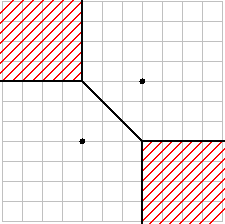
\includegraphics[width=3cm]{capture7}
\end{center}
\caption{Fall 3: $\left|\frac{x_1-x_2}{y_1-y_2}\right| =1$}
\label{fig:l1_4}
\end{figure}

Auffälig ist hier der letzte, entartete Fall, bei dem eine Menge von Punkten (rot) zu beiden Punkten equidistant ist und keine Kante sondern eine Fläche beschreibt. Wie dieser Fall im Kontext von Voronoi-Diagrammen behandelt werden sollte ist nicht aus deren Definition abzuleiten. In der Praxis sollte dieser Fall jedoch ohnehin nur relevant sein, wenn mit Ganzzahligen Koordinaten gerechnet wird.
\end{task}

\begin{task}{Suche in ebenen Unterteilungen - Verallgemeinerung}
\item[]

Die Lokalisierungsdatenstruktur (LDS) wurde in der Vorlesung als gerichteter azyklischer Graph (ADG) beschrieben und funktioniert für Triangulierung von $G$ mit Dreieck als Außenfacette.

$S_1$ entspricht $G$, also der ebenen Unterteilung  (eingebetteter Graph)
$S_n$ ist das äußere (umschließende) Dreieck

Ich habe es so verstanden dass in jedem Schritt die unabhänige Knotenmenge bestimmt und entfert wird, dass sind dann die $S_i$'s' die zwischen 1 und n konstruiert werden.

Eine Knotenmenge $I$ von $G$ (Teilmenge) heißt unabhängig, wenn keine zwei Knoten aus $I$ in $G$ durch eine Kante verbungen sind. Es geht wohl in linearer Zeit zu berechnen, weil warum auch immer, wurde in VL bewiesen.




1. vorher das Ding Triangulieren\\
2. großes Dreieck drumrum bauen\\
3. wenn ein Strahl das äußerer Dreieck schneidet, dann dort einen neuen Knoten einfügen\\
4. Eckpunkte vom Dreieck mit Punkten verbinden oder einfach nochmal Triangulieren? oder voher schon Dreicke rumbasteln

die beiden algorithmen wurden in der VL vorgestellt, diese dann noch ein bischen erweitern.

\begin{algorithm}
\caption{Algorithmus zur Konstruktion}
\begin{algorithmic}[1]
\STATE Sei $S_1=G$
\STATE Für jedes $\triangle$ in $G$ erzeuge einen Knoten in LDS($G$)
\STATE i = 1
\WHILE{$|S_i|>3$}
    \STATE{Berechne $I$}
    \STATE {Entferne $I$ aus $S_i$}
    \STATE {Trianguliere $S_i ohne I$, das ist dann $S_i+1$}
    \STATE {für jedes neue $\triangle$ $t$ in $S_i+1$ erzeuge einen Knoten K($t$)in LDS($G$), füge eine Kante von K($t$) zu allen Knoten von Dreiecken von $S_i$ die von  $t$ geschnitten werden}
    \STATE i++
\ENDWHILE
\end{algorithmic}
\end{algorithm}


h ... log(n)

\begin{algorithm}
\caption{Lokalisiere (q, LDS(G))}
\begin{algorithmic}[1]
\STATE teste ob $q \in S_h$ falls nein gib aussenfassette zurück
\STATE $v$=Wurzel(LDS(G))
\WHILE{$v$ hat Nachfolger}
    \STATE { für jeden Nachfolger von $u$ von $v$ teste ob $q$ im Dreiech $u$ liegt.}
    \STATE {Falls ja, setze $v=u$ und wiederhole}
\RETURN {$q$ liegt im Dreieck von $v$}
\ENDWHILE
\end{algorithmic}
\end{algorithm}

* Erweiterung von LDS\\
* Algorithmen zur Suche und Konstruktion anpassen\\
* alle Unterteilungen den Ebene sollen unterstützt werden (mehrere unbeschränkte Facetten)\\
* Einzelheiten der Algorithmen beschreiben\\
*Vorverarbeitungszeit, Speicherbedarf, Anfragezeit, Anhängig von Anzahl der Knoten\\ 

\end{task}
\end{document}